\documentclass[11pt,a4paper]{article}

\usepackage[margin=2.5cm]{geometry}
\usepackage{graphicx}
\usepackage{hyperref}
\usepackage{amsmath}
\usepackage{amsfonts}
\usepackage{booktabs}
\usepackage{tabularx}
\usepackage{enumitem}
\usepackage{tikz}
\usetikzlibrary{shapes,arrows,positioning,fit,calc,decorations.pathmorphing}

\title{Antenna Digital Twin: Models and Parameters\\Technical Reference}
\author{Pratik Kumar \and Shruti \and Uday Krishan Khandelwal}
\date{\today}

\begin{document}
\maketitle

\begin{abstract}
This document details the models used across the Antenna Digital Twin backend and the parameters each module consumes and produces. For each domain---Environment, Learning, Measurement, Mechanical, Optimization, and Validation---we describe \emph{what} the model does and \emph{why} it exists in the system.
\end{abstract}

\tableofcontents
\newpage

%===============================================================================
\section{System Overview}
%===============================================================================

The Antenna Digital Twin backend is organized into six main domains. The following TikZ flow illustrates how these domains interact.

\begin{figure}[htbp]
\centering
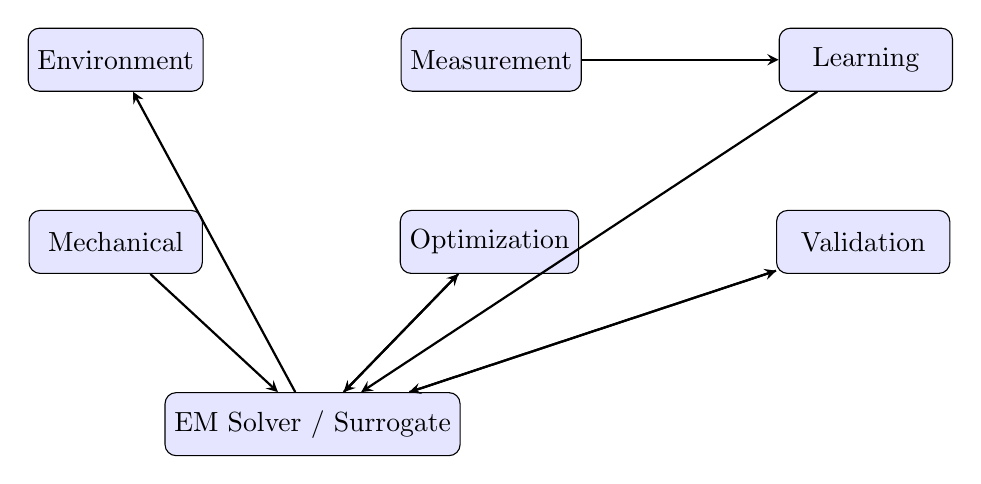
\begin{tikzpicture}[
    node distance=1.2cm,
    box/.style={rectangle, draw, rounded corners, fill=blue!10, minimum width=2.2cm, minimum height=0.8cm, align=center},
    arrow/.style={->,>=stealth, thick}
]
    \node[box] (env) {Environment};
    \node[box, right=2.5cm of env] (meas) {Measurement};
    \node[box, right=2.5cm of meas] (learn) {Learning};
    
    \node[box, below=1.5cm of env] (mech) {Mechanical};
    \node[box, right=2.5cm of mech] (opt) {Optimization};
    \node[box, right=2.5cm of opt] (val) {Validation};
    
    \node[box, below=1.5cm of mech, xshift=2.5cm] (em) {EM Solver / Surrogate};
    
    \draw[arrow] (em) -- (env);
    \draw[arrow] (meas) -- (learn);
    \draw[arrow] (learn) -- (em);
    \draw[arrow] (mech) -- (em);
    \draw[arrow] (em) -- (opt);
    \draw[arrow] (opt) -- (em);
    \draw[arrow] (val) -- (em);
    \draw[arrow] (em) -- (val);
\end{tikzpicture}
\caption{High-level flow of the six backend domains relative to EM simulation and surrogate inference.}
\end{figure}

%===============================================================================
\section{Environment}
%===============================================================================

\subsection{What}
The Environment domain models how the antenna behaves in its deployment setting: propagation loss, coverage, proximity effects (hand, housing), and orientation.

\subsection{Why}
Antenna performance depends on the operating environment. Indoor vs.\ outdoor, distance from obstacles, and mounting orientation all affect effective gain and S11. These models enable the digital twin to predict performance under real-world conditions, not just in free space.

\subsection{Models and Parameters}

\begin{table}[htbp]
\centering
\small
\begin{tabularx}{\textwidth}{@{}lXX@{}}
\toprule
\textbf{Model} & \textbf{Input / Output} & \textbf{Reason} \\
\midrule
PropagationModel & distance (m), frequency (Hz), environment $\to$ path\_loss (dB) & \emph{What}: Free-space path loss $20\log_{10}(4\pi d/\lambda)$ with optional indoor (+20\,dB) or outdoor (+10\,dB). \emph{Why}: Predicts received power at distance and environment. \\
\addlinespace
CoverageCalculator & pattern, distance, frequency, env, threshold\_gain $\to$ coverage\_prob, effective\_gain & \emph{What}: PropagationModel + max gain; checks if effective gain $>$ threshold. \emph{Why}: ``Will the link work at distance $d$?'' \\
\addlinespace
ProximityModel & parameters, obstacle\_distance, permittivity $\to$ S11 degradation factor & \emph{What}: $\exp(-d/0.02)\cdot(\varepsilon_r-1)\cdot0.1$ for $d{<}0.1$\,m; no effect $>$10\,cm. \emph{Why}: Hand/housing detunes resonance. \\
\addlinespace
OrientationModel & pattern, theta/phi rotation (deg) $\to$ RadiationPattern & \emph{What}: Placeholder for rotation. \emph{Why}: Mounting orientation affects apparent gain. \\
\bottomrule
\end{tabularx}
\caption{Environment models, parameters, and rationale.}
\end{table}

\begin{figure}[htbp]
\centering
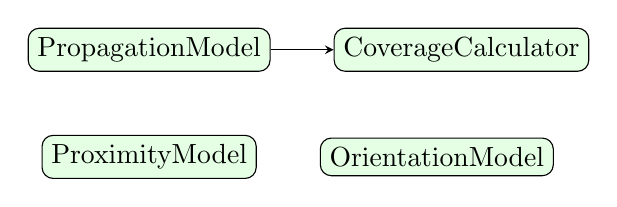
\begin{tikzpicture}[
    node distance=0.8cm,
    box/.style={rectangle, draw, rounded corners, fill=green!10, minimum width=2cm},
    arrow/.style={->,>=stealth}
]
    \node[box] (prop) {PropagationModel};
    \node[box, right=of prop] (cov) {CoverageCalculator};
    \node[box, below=of prop] (prox) {ProximityModel};
    \node[box, right=of prox] (ori) {OrientationModel};
    
    \draw[arrow] (prop) -- (cov);
\end{tikzpicture}
\caption{Environment model dependencies. Coverage uses Propagation; Proximity and Orientation act on pattern/parameters.}
\end{figure}

%===============================================================================
\section{Measurement}
%===============================================================================

\subsection{What}
The Measurement domain ingests data from VNA and chamber files, aligns it with known antenna parameters, and validates correctness.

\subsection{Why}
Physical measurements (S11, gain, efficiency) are the ground truth for calibrating the digital twin. Without reliable ingestion and alignment, learning and validation cannot use real-world data.

\subsection{Models and Parameters}

\begin{table}[htbp]
\centering
\small
\begin{tabularx}{\textwidth}{@{}lXX@{}}
\toprule
\textbf{Component} & \textbf{Input / Output} & \textbf{Reason} \\
\midrule
MeasurementIngestionService & file\_path, file\_type, antenna\_id, params, metadata $\to$ MeasurementData & \emph{What}: Parses VNA/Chamber, validates, aligns. \emph{Why}: Central entry point. \\
\addlinespace
VNAParser, ChamberParser & file path $\to$ parsed dict (freq, s11, gain, eff) & \emph{What}: Format-specific parsers. \emph{Why}: Different equipment formats. \\
\addlinespace
ParameterAligner & measurement\_data, known\_params $\to$ AntennaParameters & \emph{What}: 1\% tolerance check; aligned params. \emph{Why}: Correct design association. \\
\addlinespace
MeasurementValidator & parsed\_data $\to$ valid, errors & \emph{What}: Validates freq range, S11 bounds, fields. \emph{Why}: Reject malformed data. \\
\bottomrule
\end{tabularx}
\caption{Measurement components, parameters, and rationale.}
\end{table}

\begin{figure}[htbp]
\centering
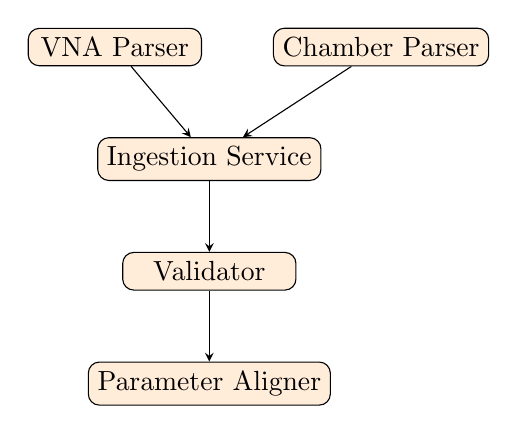
\begin{tikzpicture}[
    node distance=0.9cm,
    box/.style={rectangle, draw, rounded corners, fill=orange!15, minimum width=2.2cm},
    arrow/.style={->,>=stealth}
]
    \node[box] (vna) {VNA Parser};
    \node[box, right=of vna] (ch) {Chamber Parser};
    \node[box, below=of vna, xshift=1.2cm] (ing) {Ingestion Service};
    \node[box, below=of ing] (val) {Validator};
    \node[box, below=of val] (align) {Parameter Aligner};
    
    \draw[arrow] (vna) -- (ing);
    \draw[arrow] (ch) -- (ing);
    \draw[arrow] (ing) -- (val);
    \draw[arrow] (val) -- (align);
\end{tikzpicture}
\caption{Measurement ingestion pipeline.}
\end{figure}

%===============================================================================
\section{Learning}
%===============================================================================

\subsection{What}
The Learning domain calibrates the surrogate using measurements, performs Bayesian updates, detects drift, and triggers retraining when needed.

\subsection{Why}
The surrogate is trained on EM simulations, which can differ from physical measurements due to manufacturing tolerances, substrate variation, and environment. Learning keeps the twin aligned with reality.

\subsection{Models and Parameters}

\begin{table}[htbp]
\centering
\small
\begin{tabularx}{\textwidth}{@{}lXX@{}}
\toprule
\textbf{Model} & \textbf{Input / Output} & \textbf{Reason} \\
\midrule
CalibrationService & antenna\_id, measurement, db $\to$ discrepancy, bayesian\_update, confidence & \emph{What}: Compares pred vs.\ meas (S11, gain, eff), Bayesian update, confidence. \emph{Why}: Aligns twin with physical instance. \\
\addlinespace
BayesianUpdater & model\_pred, measurement, prior\_var $\to$ updated\_s11, variance, weight & \emph{What}: $0.7\cdot\text{meas}+0.3\cdot\text{pred}$; reduces variance. \emph{Why}: Bayesian fusion. \\
\addlinespace
DriftDetector & predictions, measurements, threshold=0.1 $\to$ drift\_detected, mean\_error & \emph{What}: Rel.\ error pred vs.\ meas S11; drift if mean $>0.1$. \emph{Why}: Detects model mismatch. \\
\addlinespace
AutomatedBayesianUpdater & antenna\_id, measurement\_id $\to$ calibration, drift\_detection & \emph{What}: Orchestrates calibration + drift on new measurement. \emph{Why}: Single entry point. \\
\bottomrule
\end{tabularx}
\caption{Learning models, parameters, and rationale.}
\end{table}

\begin{figure}[htbp]
\centering
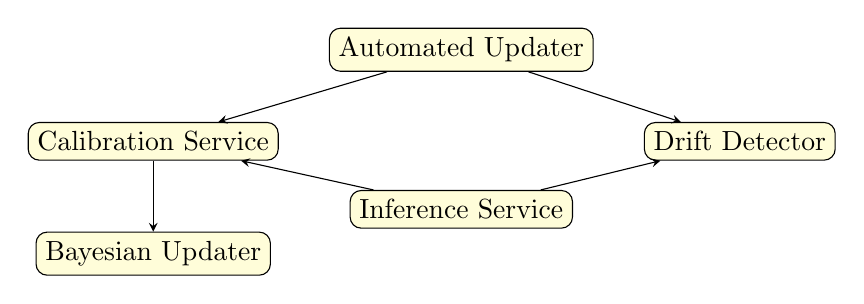
\begin{tikzpicture}[
    node distance=0.9cm,
    box/.style={rectangle, draw, rounded corners, fill=yellow!15, minimum width=2.2cm},
    arrow/.style={->,>=stealth}
]
    \node[box] (auto) {Automated Updater};
    \node[box, below left=of auto] (cal) {Calibration Service};
    \node[box, below right=of auto] (drift) {Drift Detector};
    \node[box, below=of cal] (bayes) {Bayesian Updater};
    \node[box, below=1.5cm of auto, xshift=0cm] (inf) {Inference Service};
    
    \draw[arrow] (auto) -- (cal);
    \draw[arrow] (auto) -- (drift);
    \draw[arrow] (cal) -- (bayes);
    \draw[arrow] (inf) -- (cal);
    \draw[arrow] (inf) -- (drift);
\end{tikzpicture}
\caption{Learning flow: Automated updater triggers calibration and drift detection; both use inference predictions.}
\end{figure}

%===============================================================================
\section{Mechanical}
%===============================================================================

\subsection{What}
The Mechanical domain models deformation of the antenna geometry due to bending, mounting stress, and thermal expansion.

\subsection{Why}
Flexible substrates (e.g., FR-4 on curved surfaces), mounting stress, and temperature changes alter physical dimensions and thus resonance and gain. Modeling these effects makes the twin useful for conformal and stressed designs.

\subsection{Models and Parameters}

\begin{table}[htbp]
\centering
\small
\begin{tabularx}{\textwidth}{@{}lXX@{}}
\toprule
\textbf{Model} & \textbf{Input / Output} & \textbf{Reason} \\
\midrule
BendingModel & params, bending\_radius, axis $\to$ AntennaGeometry & \emph{What}: Strain $\varepsilon=h/(2R)$; $L'=L(1+\varepsilon)$, $W'=W(1-\nu\varepsilon)$. $E=2.4$\,GPa, $\nu=0.22$. \emph{Why}: Bending changes L, W. \\
\addlinespace
StressModel & params, stress\_x, stress\_y (Pa) $\to$ AntennaGeometry & \emph{What}: $\varepsilon_x=\sigma_x/E$, $\varepsilon_y=\sigma_y/E$ + Poisson. \emph{Why}: Mounting stress stretches patch. \\
\addlinespace
ThermalExpansionModel & params, temp ($^\circ$C), $T_{\mathrm{ref}}=25$ $\to$ AntennaGeometry & \emph{What}: $1+\alpha\Delta T$, $\alpha=16\times10^{-6}$\,K$^{-1}$. \emph{Why}: Temp shifts resonance. \\
\addlinespace
GeometryDeformer & params, bending, stress, temp $\to$ AntennaParameters & \emph{What}: bending $\to$ stress $\to$ thermal sequence. \emph{Why}: Single interface. \\
\bottomrule
\end{tabularx}
\caption{Mechanical models, parameters, and rationale.}
\end{table}

\begin{figure}[htbp]
\centering
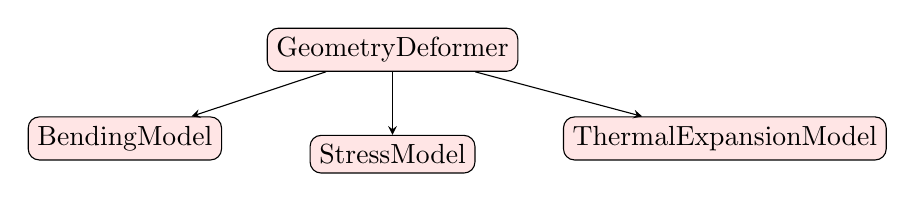
\begin{tikzpicture}[
    node distance=0.8cm,
    box/.style={rectangle, draw, rounded corners, fill=red!10, minimum width=2cm},
    arrow/.style={->,>=stealth}
]
    \node[box] (def) {GeometryDeformer};
    \node[box, below left=of def] (bend) {BendingModel};
    \node[box, below=of def] (stress) {StressModel};
    \node[box, below right=of def] (therm) {ThermalExpansionModel};
    
    \draw[arrow] (def) -- (bend);
    \draw[arrow] (def) -- (stress);
    \draw[arrow] (def) -- (therm);
\end{tikzpicture}
\caption{Mechanical deformation pipeline: GeometryDeformer chains bending, stress, and thermal.}
\end{figure}

%===============================================================================
\section{Optimization}
%===============================================================================

\subsection{What}
The Optimization domain tunes antenna geometry to meet targets: single-value S11, full S11 spectrum (UCE-style), and what-if analysis.

\subsection{Why}
Engineers need to find geometries that achieve desired S11, gain, or efficiency. Single-target optimization (e.g., S11 = $-10$\,dB) is common; spectrum matching supports multi-band and measured-target workflows. What-if analysis explores sensitivity without running full optimization.

\subsection{Models and Parameters}

\begin{table}[htbp]
\centering
\small
\begin{tabularx}{\textwidth}{@{}lXX@{}}
\toprule
\textbf{Model} & \textbf{Input / Output} & \textbf{Reason} \\
\midrule
GeometryOptimizer.optimize\_s11 & initial\_params, target\_s11 (dB), bounds $\to$ AntennaParameters & \emph{What}: L-BFGS-B on surrogate; min $|$s11\_min $-$ target$|$. \emph{Why}: Gradient-based single target. \\
\addlinespace
optimize\_s11\_spectrum & initial, target\_freq/s11\_db, optimizer, quantile, n\_samples, elite\_frac, n\_iter $\to$ params, loss\_history & \emph{What}: UCE spectrum loss + L-BFGS-B or CEM. \emph{Why}: Match full S11 curve. \\
\addlinespace
spectrum\_loss & pred/target freq and S11\_db, quantile $\to$ scalar & \emph{What}: Piecewise loss (squared/mixed L1), quantile threshold. \emph{Why}: Robust; UCE design. \\
\addlinespace
cross\_entropy\_optimize & func, bounds, n\_samples, elite\_frac, n\_iter $\to$ best\_x, score, history & \emph{What}: CEM uniform sampling; elite updates dist. \emph{Why}: Derivative-free. \\
\addlinespace
WhatIfAnalyzer & base\_params, variation $\to$ Dict[str, SurrogatePrediction] & \emph{What}: Surrogate for base + varied params. \emph{Why}: Sensitivity exploration. \\
\bottomrule
\end{tabularx}
\caption{Optimization components, parameters, and rationale.}
\end{table}

\begin{figure}[htbp]
\centering
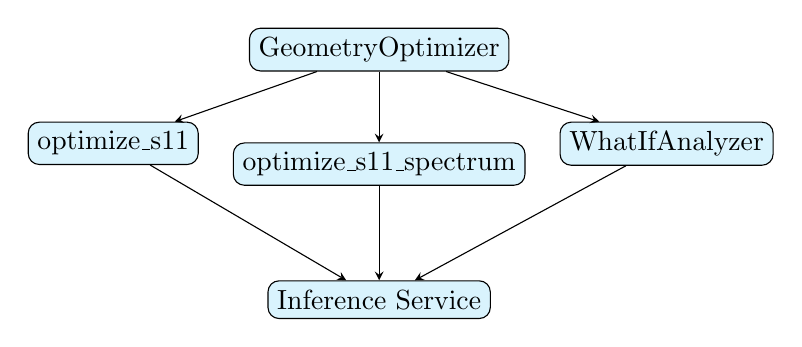
\begin{tikzpicture}[
    node distance=0.9cm,
    box/.style={rectangle, draw, rounded corners, fill=cyan!15, minimum width=2cm},
    arrow/.style={->,>=stealth}
]
    \node[box] (opt) {GeometryOptimizer};
    \node[box, below left=of opt] (s11) {optimize\_s11};
    \node[box, below=of opt] (spec) {optimize\_s11\_spectrum};
    \node[box, below right=of opt] (wif) {WhatIfAnalyzer};
    \node[box, below=1.2cm of spec] (inf) {Inference Service};
    
    \draw[arrow] (opt) -- (s11);
    \draw[arrow] (opt) -- (spec);
    \draw[arrow] (opt) -- (wif);
    \draw[arrow] (s11) -- (inf);
    \draw[arrow] (spec) -- (inf);
    \draw[arrow] (wif) -- (inf);
\end{tikzpicture}
\caption{Optimization flows. All use Inference Service (surrogate) for fast evaluations.}
\end{figure}

%===============================================================================
\section{Validation}
%===============================================================================

\subsection{What}
The Validation domain compares surrogate predictions to EM ground truth and tracks KPIs over time.

\subsection{Why}
Surrogates must stay within acceptable error bounds. Validation quantifies MAE, RMSE, R$^2$, and max error so engineers know when to retrain or trust predictions.

\subsection{Models and Parameters}

\begin{table}[htbp]
\centering
\small
\begin{tabularx}{\textwidth}{@{}lXX@{}}
\toprule
\textbf{Model} & \textbf{Input / Output} & \textbf{Reason} \\
\midrule
EMSurrogateValidator & em\_results, surrogate\_preds, metric $\to$ MAE, MRE, RMSE, max\_err, R2 & \emph{What}: EM vs.\ surrogate comparison. \emph{Why}: Surrogate accuracy. \\
\addlinespace
KPITracker & kpi\_name, value, metadata $\to$ JSON file & \emph{What}: Logs KPIs with timestamp. \emph{Why}: Track metrics over time. \\
\bottomrule
\end{tabularx}
\caption{Validation components, parameters, and rationale.}
\end{table}

%===============================================================================
\section{Core Parameters and Schemas}
%===============================================================================

\subsection{AntennaParameters}
The central input to EM simulation, surrogate inference, mechanical deformation, and optimization.

\begin{table}[htbp]
\centering
\small
\begin{tabularx}{\textwidth}{@{}lXl@{}}
\toprule
\textbf{Field} & \textbf{Type} & \textbf{What \& Why} \\
\midrule
geometry.length & float (m) & Patch length $L$; resonance. \\
geometry.width & float (m) & Width $W$; bandwidth. \\
geometry.height & float (m) & Substrate $h$; $Q$, bandwidth. \\
geometry.feed\_x, feed\_y & float (m) & Feed; impedance match. \\
substrate.substrate\_type & FR4, RO4003, RO4350 & Material; $\varepsilon_r$, tan~$\delta$. \\
substrate.relative\_permittivity & float & $\varepsilon_r$; resonance. \\
substrate.loss\_tangent & float & tan~$\delta$; losses. \\
frequency\_band & 2.4GHz, 3.5GHz & Band; default freq range. \\
frequency\_range & (f\_min, f\_max) Hz & Sim/pred frequency span. \\
\bottomrule
\end{tabularx}
\caption{AntennaParameters schema.}
\end{table}

\subsection{Surrogate Model Parameters}
The ensemble combines GP and NN; features are the 7 antenna parameters (length, width, height, feed\_x, feed\_y, $\varepsilon_r$, tan~$\delta$). Target metrics: \texttt{s11\_min}, \texttt{gain}, \texttt{efficiency}.

\begin{table}[htbp]
\centering
\small
\begin{tabularx}{\textwidth}{@{}lXX@{}}
\toprule
\textbf{Model} & \textbf{Key Parameters} & \textbf{What \& Why} \\
\midrule
GaussianProcessSurrogate & input\_dim=7, Matern($\nu=2.5$) & GP with uncertainty; confidence intervals. \\
NeuralSurrogate & input\_dim=7, hidden [64,128,64], dropout 0.2 & MLP; fast inference, scales to more data. \\
EnsemblePredictor & weighted\_avg (0.6 GP, 0.4 NN) & Blends GP+NN; GP for uncertainty. \\
\bottomrule
\end{tabularx}
\caption{Surrogate model parameters.}
\end{table}

%===============================================================================
\section{Configuration (Settings)}
%===============================================================================

Key configuration values that affect behavior:

\begin{table}[htbp]
\centering
\small
\begin{tabularx}{\textwidth}{@{}lXX@{}}
\toprule
\textbf{Setting} & \textbf{Default} & \textbf{What \& Why} \\
\midrule
ML\_MODEL\_DIR & models/ & Surrogate pickles. \\
ML\_DEVICE & cpu & PyTorch device; cuda for GPU. \\
EM\_SOLVER\_TIMEOUT & 3600 s & Max sim time per run. \\
EM\_SOLVER\_MAX\_WORKERS & 4 & Parallel EM for batch training. \\
POSTGRES\_* & localhost, 5432, antenna\_twin & Database for instances, measurements. \\
\bottomrule
\end{tabularx}
\caption{Key configuration parameters.}
\end{table}

%===============================================================================
\section{Conclusion}
%===============================================================================

This report documented the models and parameters used in the Antenna Digital Twin backend. Each domain---Environment, Measurement, Learning, Mechanical, Optimization, and Validation---has a clear role: Environment models deployment conditions; Measurement ingests and aligns physical data; Learning calibrates and detects drift; Mechanical models deformation; Optimization tunes geometry; Validation ensures surrogate accuracy. The core parameters (AntennaParameters, surrogate features, and configuration) are defined to support 2.4\,GHz and 3.5\,GHz microstrip patch antenna twinning with minimal coupling between modules.

\end{document}
